\chapter{Microsoft DirectCompute}
\label{chap:DirectCompute}

 
Resources:
\begin{enumerate}
  \item
  \url{http://msdn.microsoft.com/en-us/library/windows/desktop/ff476331(v=vs.85).aspx}
  \item
  \url{http://blogs.msdn.com/b/chuckw/archive/2010/07/14/directcompute.aspx}
\end{enumerate}

Nowadays, with a normal 4-core CPU, each core can do 4 floating-point
operations simultaneously per clock (i.e. 4 float-wide SIMD) with speed 48-96
GFLOPS (single-precision math). A typical GPU can have about 32 ``cores'' (SIMD
engines). Each SIMD engine can do 32 floating-wide operations per clock, which
can deliver 1 TFLOPs (single-precision). The main design difference:
\begin{itemize}
  \item CPU: handle large random access (20 GB/s bandwidth) with wide-known
  programming model
  \item GPU: handle sequential access (100 GB/s bandwidth) with less common
  programming model. So, localization is very important
\end{itemize}
We knowaday consider a PC as an assymmetric multi-processor systems (with
CPU-CPU, or CPU-GPU); but in many cases, the bandwith between CPU-GPU is slower
than the front-side bus, Fig.\ref{fig:GPU_CPU_system}.

\begin{figure}[hbt]
  \centerline{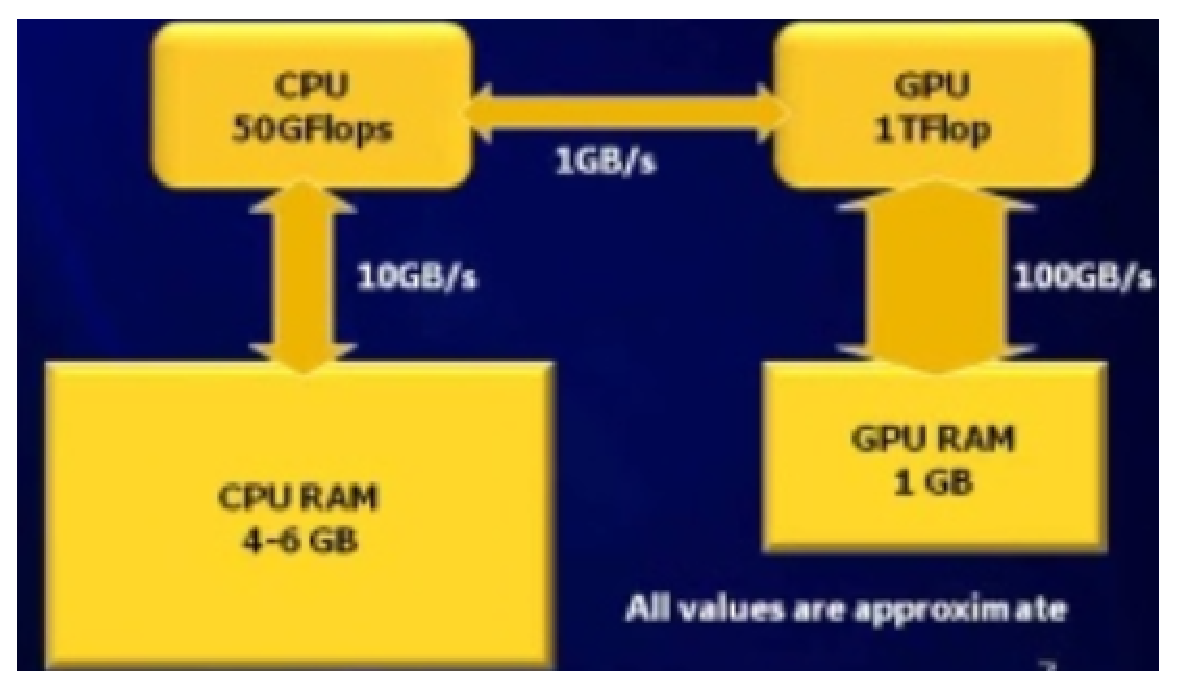
\includegraphics[height=5cm,
    angle=0]{./images/GPU-CPU.eps}}
  \caption{GPU-CPU assymetric multi-processor system}
  \label{fig:GPU_CPU_system}
\end{figure}

\section{Introduction}

DirectCompute was developed by Microsoft, directly on top of the processor, at
the same level of CUDA, OpenCL. GPU is recognized as a viable floating-point
accelerator. All DirectX11 chips, and some DirectX10 chips, will support
DirectCompute. \textcolor{blue}{As DirectCompute is built on DirectX
technologies, a good understanding of DirectX is recommended}.

DirectX10 was limited to Windows Vista only. Soon after that, Microsoft
introduced DirectX 11 which is a huge step forwards, with more complex shaders
(Vertex, Hull, Domain, Geometry, Pixel and Compute Shaders) and new tricks like
tessellation hardward units. Prominent new features in DirectX 11,
Fig.\ref{fig:DirectX_comparison}:
Shader model 5.0 (Sect.\ref{sec:shader_model}), Multi-threaded rendering,
DirectCompute 11, Hardware Tessellation (Sect.\ref{sec:tessellation}), Better
shadows, HDR Texture compression (Sect.\ref{sec:HDR_Texture_compression}).


\begin{figure}[hbt]
  \centerline{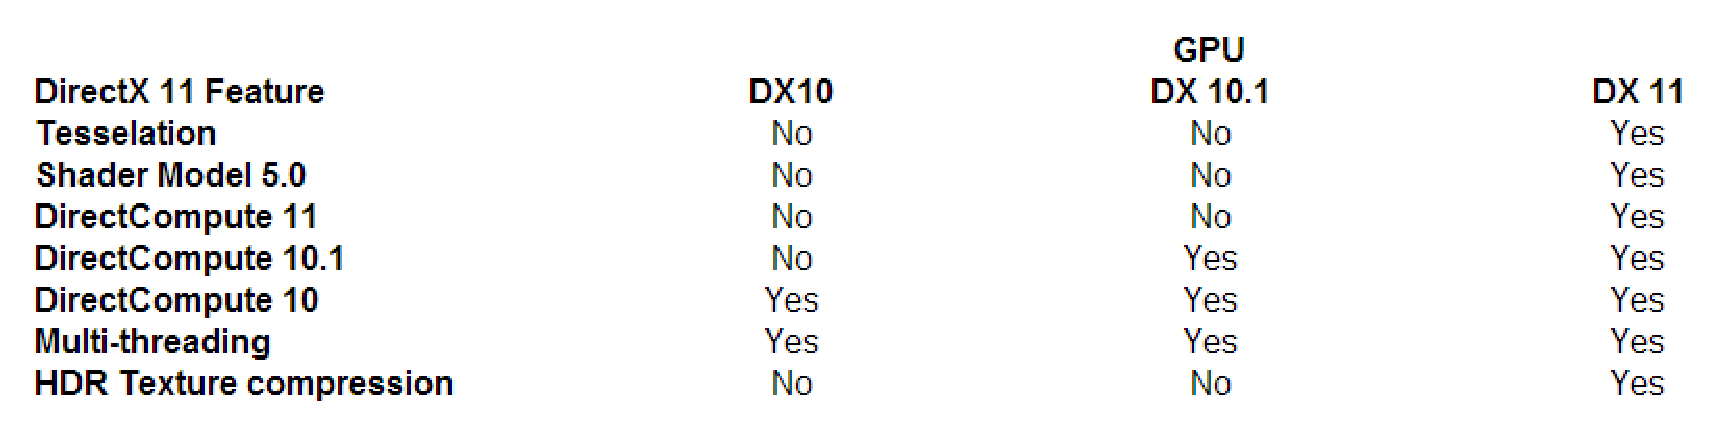
\includegraphics[height=3cm,
    angle=0]{./images/DirectX_comparison.eps}}
  \caption{DirectX 10, DirectX 11 comparison}
  \label{fig:DirectX_comparison}
\end{figure}

DirectCompute has potentially use in Physics, AI, image processing and filtering
(post processing), order independent transparency (a really cool feature where
you could see through an object like it was made out of glass), shadows
rendering. As the program may want direct rendering, DirectCompute has tight
integration with rendering. So, the techniques can be widely used in Game
Technologies (Rendering, etc.). It also support media data-types, with hardware
format conversion for pixel formats.


\section{Write the code}

We need to initialize API.
\begin{verbatim}
hr = D3D11CreateDevice( ...)
\end{verbatim}
The code need to be written in .hlsl language, and compile using DirectX
compiler. The example code in HLSL is similar to C++
\begin{verbatim}
#define BLOCK_SIZE 256

StructureBuffer gBuf1 : register(t0);
StructureBuffer gBuf2 : register(t1);

RWStructureBuffer gBufOut : register(u0);

[numthreads(BLOCK_SIZE, 1, 1)] void VectorAdd (uint3 id: SV_DispatchThreadID )
{
  gBufOut[id] = gBuf1[id] + gBuf2[id];
}
\end{verbatim}
It load code onto the GPU, set up a GPU buffer for input data, set up a view
into it for access. We make that data view current, and execute the code on GPU.
Finally, data is copied back to CPU memory. 

\begin{framed}
A {\bf dispatch} is a set of work launched as an atomic operation. This is aka
'grid' (or set of thread groups).

A {\bf thread group} is a set of threads assigned to a specific SIMD engine.
This is aka 'thread block' (NVdia) or 'work group' (AMD).

A {\bf thread vector} is a set of threads all executed in lockstep on a single
SIMD core. This is aka ``warp''. 

A {\bf resource} is a segment of memory allocated for use by the GPU.

A {\bf view} is an interface on a Resource that define the structure of the data
so that we know how to access it.
\end{framed}

\section{HLSL}

HLSL is similar to C, like
\begin{enumerate}
  \item preprocessor (\verb!#define!, \verb!#ifdef!, etc.)
  \item basic types (float, int, uint, bool)
  \item operators, variables, functions
\end{enumerate}

HLSL has 
\begin{enumerate}
  \item NO support for pointers
  \item built-in variables and types, e.g. float4, matrix, etc.
  \item its own intrinsic functions (mul, normalize, etc.)
\end{enumerate}

\subsection{HLSL compiler}

It has two-stage approach. As shown in Fig.\ref{fig:HLSL_compile}, the HLSL
compiler is command-line {\bf fxc} or library to generates codes in IL
from shader. Shader Intermediate Language (IL) is defined by Microsoft with very
high optimization code.  Then, driver component translates to final instruction set.

\begin{verbatim}
hr = D3DX11CompileFromFile(
  "mycode.hlsl", //path to the .hlsl file
  NULL,
  NULL,
  "vectorAdd", //entry point
  pProfile,
  D3D10_SHADER_ENABLE_STRICTNESS,
  NULL,
  NULL,
  &pBlob, //compiled shader
  &pErrorBlob, //error log
  NULL
 );

\end{verbatim}

\begin{figure}[hbt]
  \centerline{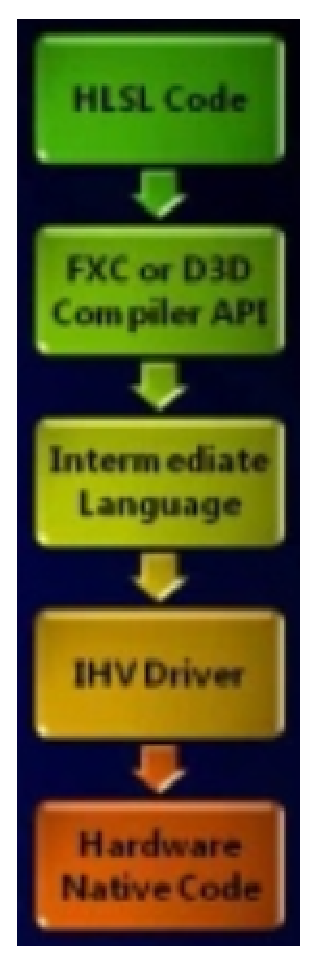
\includegraphics[height=7cm,
    angle=0]{./images/HLSL_compile-stages.eps}}
  \caption{Phases in compiling HLSL}
  \label{fig:HLSL_compile}
\end{figure}

Once the IL shader was compiled, we can actually create the shader handle
\begin{verbatim}
pD3D->CreateComputeShader( pBlob->GetBufferPointer(),
   pBlob->GetBufferSize(),
   NULL,
   &pMyShader );

pD3D->CSSetShader ( pMyShader,
   NULL,
   0
 );
\end{verbatim}

\subsection{Create Buffer}  

We define a range of memory to be considered as input
\begin{verbatim}
D3D11_BUFFER_DESC descBuf;

ZeroMemory( &descBuf, size(descBuf));

desc.BindFlags = D3D11_BIND_UNORDERED_ACCESS;
desc.StructureBytesStride = uElementSize;
desc.ByteWidth = uElementSize * uCount;
desc.MiscFlags = D3D11_RESOURCE_MISC_BUFFER_STRUCTURED;

pD3D->CreateBuffer( &desc, pInput, ppBuffer);
\end{verbatim}

\subsection{Resource Objects/Resource Views}

The relationship between buffers and views,
Fig.\ref{fig:DirectCompute_BufferView}. Resource Objects are used to store data;
while Resource Views are interfaces to the Resource Objects.

\begin{figure}[hbt]
  \centerline{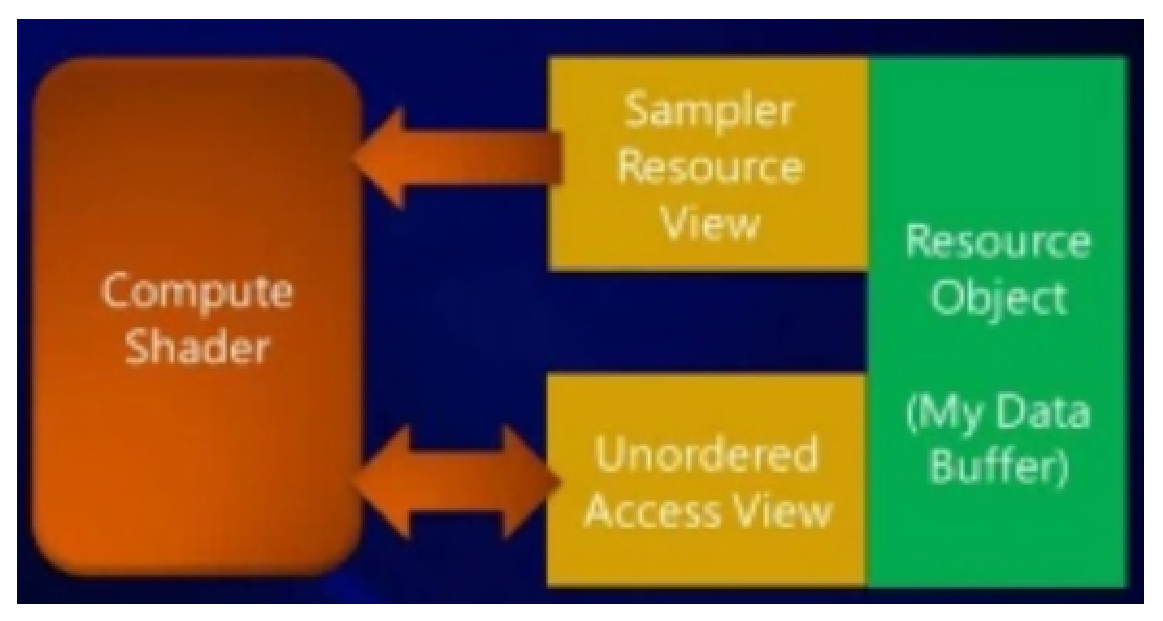
\includegraphics[height=4cm,
    angle=0]{./images/DirectCompute_BufferView.eps}}
  \caption{Buffers vs. Views in DirectCompute}
  \label{fig:DirectCompute_BufferView}
\end{figure}

% \section{Unordered-access view}

Only one unordered-access view can be bound to the compute shader
\begin{verbatim}
D3D11_CS_4_X_UAV_REGISTER_COUNT
\end{verbatim}

\subsection{DirectX Resources}

DirectX Resources define Data Objects in memory, with support
\begin{itemize}
  \item enable out-of-bound memory checking to improve security, reliability of
  the code, return 0 on reads, and writes are no-ops. Any attempt to write out
  of that range is ignored by the implementation.
  \item facilitates interop with Direct3D for display.
\end{itemize}

There are 2 types of DirectX Resource
\begin{enumerate}
  \item Buffer: a sequence of data records, arbitrary data struct for the
  records
  \item Texture: designed for storage data to be used in pixel tasks, e.g. 1D,
  2D and 3D textures, cube maps and arrays.
  
  \item Structured: a record size with a fixed size, pixel dta format isnot
  specified
\end{enumerate}

To execute an instruction on GPU, we call 
\begin{verbatim}
ID3D11DeviceContext::Dispatch or ID3D11DeviceContext::DispatchIndirect 
\end{verbatim}

The maximum number of threads per group is defined in (default:768) 
\begin{verbatim}
D3D11_CS_4_X_THREAD_GROUP_MAX_THREADS_PER_GROUP 
\end{verbatim}

A compute shader can run many threads in parallel. Threads are organized in 2D,
with the X and Y dimension of {\bf numthreads} is limited by the value defined
in (default: 768) [NOTE: The Z dimension is limited to 1]
\begin{verbatim}
 D3D11_CS_4_X_THREAD_GROUP_MAX_X 
 D3D11_CS_4_X_THREAD_GROUP_MAX_Y
\end{verbatim}

The Z dimension of dispatch is limited by the value defined in (default: 1)
\begin{verbatim}
D3D11_CS_4_X_DISPATCH_MAX_THREAD_GROUPS_IN_Z_DIMENSION 
\end{verbatim}


\section{Double-precision}

To test if the device support double-precision, we need check the flag
\begin{verbatim}
D3D11_FEATURE_DOUBLES
\end{verbatim}
of \verb!D3D11_FEATURE! enumeration.
